\section{Mit eignenen Modellen ergänzte Sensordaten}
Im Projekt ist die Sensorenbox potentiell mit einem Accelerometer, Gyroskop, Lichtsensor, Magnetfeldsensor,
Temperatursensor und Geräuschsensor ausgestattet, sowie einen Empfänger zur Erfassung von WLAN-Zugangspunkten.
Mit CoppeliaSim ist es allerdings nur möglich Sensorwerte des Accelerometers, Gyroskops und Lichtsensors zu erfassen.
Aus diesem Grund werden die fehlenden Sensoren durch das Ausnutzen vereinfachter Modelle ergänzt.

\subsection{Magnetfeldsensor}
Magnetfeldsensoren messen das Magnetfeld auf Basis von Effekten die dadurch induziert werden, z. B. die Lorentzkraft oder der Hall-Effekt \cite{thompsonMEMS}.
Eine Anwendung dieses Sensors ist der Kompass.
Dieser richtet sich nach dem Magnetfeld der Erde aus und wird daher traditionell zur Navigation verwendet.
\newline
\newline
Das vereinfachte Modell des simulierten Magnetfeldsensors fungiert wie ein Kompass.
Die Ausgabe ist der relative Richtungsunterschied von der Sensorenbox zum magnetischen Nordpol.
Dabei können starke magnetische Objekte in der Umgebung Einfluss auf den Sensor haben,
sodass sich der magnetische Nordpol für den simulierten Sensor ändern kann.
Die Ausgabewerte sind zwischen 0 und 359, d. h. 0 ist Norden, 90 Osten, 180 Süden und 270 Westen.
\newline
\newline
Es wird angenommen, dass der magnetische Nordpol der Erde weit genug weg ist,
sodass sich im Fabrikszenario die Richtung nur ändern kann, wenn die Ausrichtung der Sensorenbox geändert wird
oder, wenn ein magnetisches Objekt in der Umgebung Einfluss ausübt.
Außerdem wird angenommen, dass sich die Ausrichtung des Objektes in einem Zyklus nicht ändert,
da Fließbandsysteme für gewöhnlich nicht rund sind, sondern Kante auf Kante aufeinander übergehen.
Allerdings wird für jeden Zyklus eine neue zufällige Ausrichtung zwischen 0 und 359 gewählt,
da das Objekt mit verschiedenen Ausrichtungen auf das Fließband gelegt werden könnte.
Zudem wird keine Interferenz der magnetischen Objekte zueinander angenommen.
Sollten sie sich überschneiden wird das magnetische Objekt mit dem meisten Einfluss gewählt.
\newline
\newline
Starke magnetische Objekte sind strategisch in der Umgebung des Fließbandsystems plaziert.
Ihre Stärke wird dabei durch die Einflussreichweite definiert, wobei der Einfluss quadratisch mit der Distanz abnimmt.
Ist der Einfluss bei 100\%, so wird für den magnetischen Nordpol die Position des magnetischen Objekts angenommen.
Wenn der Einfluss geringer ist, dann wird ein magnetischer Nordpol zwischen dem magnetischen Nordpol der Erde und des magnetischen Objektes Anteilweise gewählt.
Die magnetischen Objekte können unterschiedliche Einflussreichweiten haben.
\newline
\newline
Abbildung \ref{fig:magnetic_model} illustriert diese Situation.
Um die Ausrichtung der Sensorenbox relativ zum magnetischen Nordpol der Erde bei 0 und dem Einfluss des magnetischen Objekts zu berechnen,
ist es nötig die Winkel zwischen dem magnetischen Nordpol der Erde und dem magnetischen Objekt, sowie den Winkel zur Sensorenbox zu wissen.
Der Winkel $\beta$ vom magnetischen Nordpol der Erde zur Sensorenbox $p_{o}$ ist bekannt.
Der Winkel $\gamma$ vom magnetischen Nordpol der Erde zum magnetischen Objekt $p_{m}$ wird aus dem Winkel $\alpha$ innerhalb des eigenen Quadranten
und der Anzahl der Quadranten, zum Quadranten in dem sich $p_{m}$ befindet, berechnet.
Dabei werden die Quadranten im Uhrzeigersinn gezählt.
\begin{figure}[h!]
    \centering
    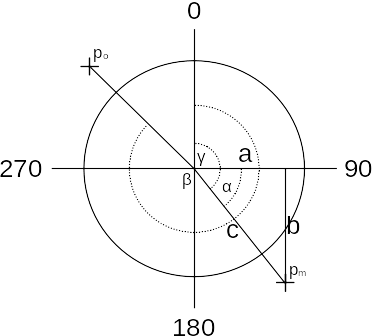
\includegraphics[width=0.7\linewidth]{images/magnetic_model.png}
    \caption{Ausrichtung der Sensorenbox relativ zum magnetischen Objekt und magnetischen Nordpol der Erde.}
    \label{fig:magnetic_model}
\end{figure}
Je nach Quadrant können für $a$ und $b$ die $x$- bzw. $y$-Koordinate von $p_{m}$ gewählt werden.
Da der Einfluss des magnetischen Objekts $p_{m}$ abhängig von der Position der Sensorenbox $p_{o}$ ist,
müssen $a$ und $b$ mit $p_{o}$ als Ursprung transformiert werden.
Die Berechnung von $\alpha$ folgt dann Formel \ref{formular:magnetic_sensor_alpha}.
\begin{align}
    \label{formular:magnetic_sensor_alpha}
    \alpha = \arcsin (\frac{|p_{o_a} - p_{m_a}|}{\sqrt{(p_{o_a} - p_{m_a})^2 + (p_{o_b} - p_{m_b})^2}})
\end{align}
Mit den Winkeln $\gamma$ und $\beta$ kann dann das Koordinatensystem zum magnetischen Objekt hin rotiert werden,
sodass die Ausrichtung von $p_{o}$ zum beeinflussten magnetischen Nordpol aus Formel \ref{formular:magnetic_sensor_new_heading} berechnet werden kann.
\begin{align}
    \label{formular:magnetic_sensor_new_heading}
    \gamma^{\prime} = (\gamma + (360 - \beta))\mod 360
\end{align}
Zu beachten ist schließlich der Einfluss $\eta$, der abhänging von der Distanz von $p_{m}$ zu $p_{o}$ ist.
Formel \ref{formular:magnetic_sensor_influence} modelliert den Einfluss als quadratisch abfallende Funktion mit zunehmender Distanz $d$ und maximaler Einflussdistanz $d_{\max}$,
wobei der maximale Einfluss 1 ist und der minimale Einfluss 0 ist.
\begin{align}
    \label{formular:magnetic_sensor_influence}
    \eta(d) = \min(0, 1 - \frac{d^2}{d_{\max}^2})
\end{align}
Der Einfluss wirkt sich proportional auf den Winkel von $p_{m}$ zum magnetischen Nordpol der Erde aus.
Dabei ist aber die Ausrichtung von $p_{m}$ zum magnetischen Nordpol der Erde zu beachten, denn bei den Polen des Magnetfeldes ändert sich die Richtung des Magnetfeldes.
Formel \ref{formular:magnetic_sensor_end_result} zeigt die Berechnung von $\gamma^{\prime}$ abhänging von der Ausrichtung von $p_{m}$ zum magnetischen Nordpol der Erde,
wobei $d = \sqrt{(p_{o_a} - p_{m_a})^2 + (p_{o_b} - p_{m_b})^2}$.
\begin{align}
    \label{formular:magnetic_sensor_end_result}
    \gamma^{\prime}_L = (\gamma + (360(1 + \eta(d)) - \beta(1 - \eta(d))))\mod 360 \\\nonumber
    \gamma^{\prime}_R = (\gamma + (360 - \beta(1 - \eta(d))))\mod 360 \hspace{0.8cm}
\end{align}

\subsection{Temperatursensor}
Das vereinfachte Modell für diesen Sensor geht von einer konstanten Umgebungstemperatur aus.
Im Raum sind Wärmequellen strategisch verteilt, die eine Temperatur unterhalb und oberhalb der Umgebungstemperatur haben können.
Je näher sich die Sensorenbox an einer der Wärmequellen befindet, desto mehr nähert sich die gemessene Temperatur der Temperatur der Wärmequelle $T_{\max}$ an.
\newline
\newline
Jede Wärmequelle hat einen Einflussbereich, in der sie sich auf die Umgebungstemperatur $T_U$ auswirken kann.
Sollten sich zwei Wärmequellen überschneiden wird die Temperatur ausgewählt, die den größten Unterschied zur Umgebungstemperatur verursacht.
Formel \ref{formular:temperature_sensor_temperature} zeigt die Berechnung der resultierenden Temperatur $T^{\prime}$ abhängig von der Distanz $d$ der
Wärmequelle zur Sensorenbox und der maximalen Einflussdistanz $d_{\max}$.
\begin{align}
    \label{formular:temperature_sensor_temperature}
    T^{\prime} = \begin{cases}
                     T_U & \text{, wenn } d > d_{\max} \\
                     \frac{(T_{\max} - T_U)d^2}{d_{\max}} + T_U & \text{, ansonsten}
    \end{cases}
\end{align}

\subsection{Geräuschsensor}
Es gibt verschiedene Arten von Geräuschsensoren, z. B. Geräuschrichtungssensoren \cite{tiete2014soundcompass} oder
spezifische Anwendungen, wie Herzgeräuschsensoren \cite{zhang2016design}.
Das Modell ist einem Akustiksensor \cite{sessler1991acoustic}, oder einem Mikrophone am ähnlichsten,
dass die Lautstärke in einem Frequenzbereich misst.
\newline
\newline
In diesem Modell werden Frequenzbereiche vernachlässigt.
Es gibt ein Hintergrundrauschen $V_H$, auf das für jeden Datensatz ein zufälliges Rauschen addiert wird.
Daneben gibt es Lautstärkequellen, die entweder periodisch oder konstant sind und strategisch im Raum verteilt sind.
Die Interferenz von verschiedenen Lautstärkequellen wird vernachlässigt.
Sollten sich zwei Lautstärkequellen überschneiden, so wird die maximale Lautstärke ausgewählt.
\newline
\newline
Die Lautstärke $V_{\max}$ die von einer Quelle ausgeht nimmt quadratisch mit der Distanz $d$ ab.
Dabei wird der Einflussbereich von der maximalen Einflussdistanz $d_{\max}$ bestimmt.
Formel \ref{formular:sound_sensor_constant_sound} zeigt die Berechnung für die resultierende Lautstärke durch eine konstante Lautstärkequelle.
\begin{align}
    \label{formular:sound_sensor_constant_sound}
    V^{\prime} = \begin{cases}
                     V_H & \text{, wenn } d > d_{\max} \\
                     \frac{(V_{\max} - V_H)d^2}{d_{\max}} + V_H & \text{, ansonsten}
    \end{cases}
\end{align}
Periodische Lautstärkequellen emittieren ein Geräusch in regelmäßigen Abständen.
Dies wird modelliert durch eine quadratisch verringerde Lautstärke über 500 ms,
wenn die Lautstärke gemessen wird nachdem das Geräusch stattgefunden hat,
d. h. nach 500 ms, ist das Geräusch nicht mehr wahrzunehmen.
Formel \ref{formular:sound_sensor_periodic_sound} beschreibt diesen Zusammenhang,
wobei $t$ der momentane Zeitpunkt ist und $t_{n}$ das Interval des periodischen Geräusches ist.
\begin{align}
    \label{formular:sound_sensor_periodic_sound}
    \hspace{-0.4cm}
    V^{\prime} = \begin{cases}
                     V_H & \text{, wenn } d > d_{\max} \vee t\ \text{mod}\ t_{n}\leq 0,5 \\
                     \max(V_H, (\frac{(V_{\max} - V_H)d^2}{d_{\max}} + V_H)(1 - 4(t\ \text{mod}\ t_{n})^2)) & \text{, ansonsten}
    \end{cases}
\end{align}

\subsection{WLAN-Zugangspunkte}
Die Detektierung von WLAN-Zugangspunkten ist eine Konsequenz aus der Detektierung von RSSI-Werten bzw. MAC-Adressen von WLAN-Zugangspunkten.
Das Modell vereinfacht dies, indem es lediglich aussagt, ob ein WLAN-Zugangspunkt in Reichweite ist oder nicht.
\newline
\newline
Im Raum sind strategisch WLAN-Zugangspunkte verteilt.
Diese können innerhalb einer maximalen Reichweite empfangen werden.
Ist die Distanz der Sensorenbox zum WLAN-Zugangspunkt innerhalb der Reichweite, gilt der WLAN-Zugangspunkt als empfangen.
Interferenzen und Reflektionen werden vernachlässigt.